\section{The \emph{Model} Level: A Domain-Specific Requirements Gathering
Framework in Action}
\label{sec:model}
\vspace{-.5cm}
We will now exemplify how a user, in this case a \emph{requirements engineer},
can make use of the specialized requirements framework we have defined in section~\ref{sec:custom_frame}.
In particular, based on an existing requirements document provided by Diehl
Aerospace and following the directions made available to us from engineers at
Diehl, we will incrementally build the requirements for the software that
controls a fan-based cooling system to cool down hardware boards embedded in
the doors of passenger airplanes.
Because of the fact that airplane doors include slides that should only be
deployed when a plane lands under specific conditions, the logic running in
those boards is non-trivial. The goal of the controller is to make
sure the cooling fan runs at the correct duty cycle (fan speed) such that the 
the hardware board works under ideal temperature conditions. The calculation of
the duty cycle for the fan at a given time depends on two inputs:
1) the current temperature of the hardware board that needs cooling and 2);
whether the hardware board's temperature is increasing or decreasing.
 
% In the text that follows we will describe how to build the requirements for the
% fan controller software using the framework defined in section~\ref{sec:model}.
% This will be achieved by starting from an abstract requirement containing only a
% natural-language description of the fan's operation, and then performing a
% set of tool-guided and tool-supported refinements that in the end lead to a description
% of the expected behavior of the fan cooling system as a function.

Note that in the example that follows we do not pretend to be exhaustive in the
construction of the requirements for the fan's controller. This section
reflects part of our partners' requirements refinements process and demonstrates
our framework's abilities in terms of providing automated assistance to the
requirements engineer. 
\vspace{-.3cm}
\subsection*{Tool Supported Requirements Definition and Refinement}
\vspace{-.3cm}
The first thing to do in a requirements project for a cooling controller is to
create a new dashboard as part of the requirements model being built. This is
achieved by instantiating the \textsf{dashboard} concept that implements the
process depicted in figure~\ref{fig:flow_statechart}. A newly generated
dashboard for our fan requirements project is depicted in figure~\ref{fig:empty_dashboard}.
\vspace{-.6cm}
\begin{figure*}[!h]
\centering 
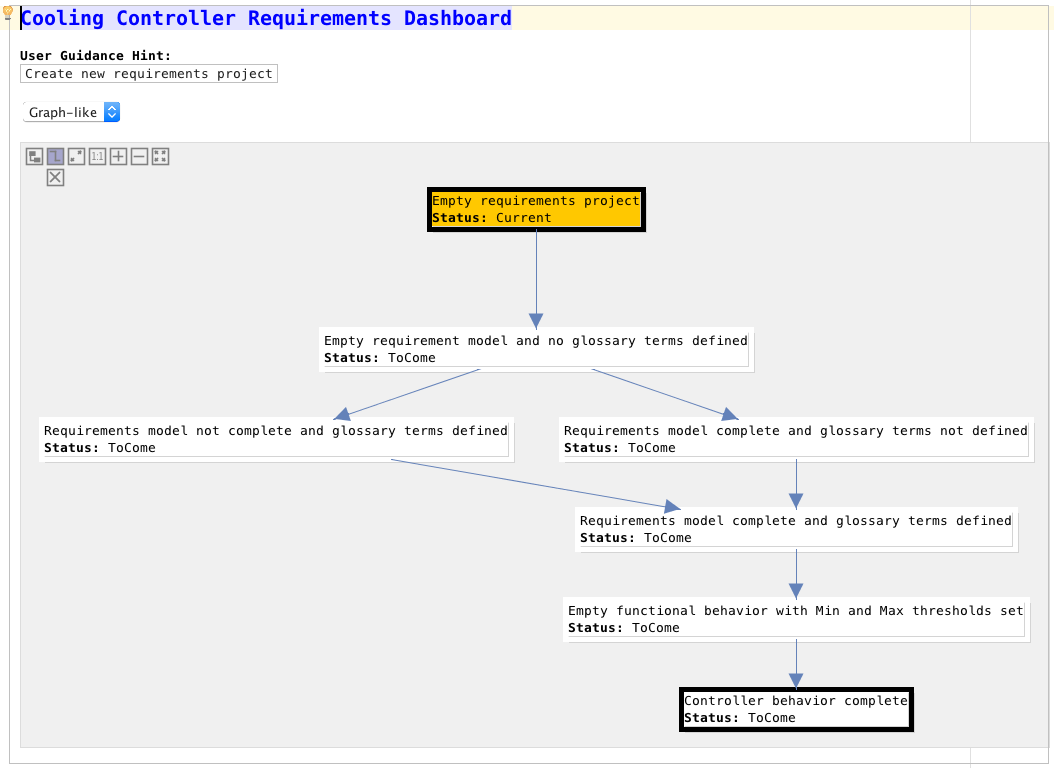
\includegraphics[width=.8\textwidth]{./figures/NewDashboard.png}
\caption{A newly created dashboard for the requirements framework}
\label{fig:empty_dashboard}
\vspace{-.6cm}
\end{figure*}
The dashboard is the central artefact the requirements engineer refers to during
requirements construction. It displays the current hint given to the
\emph{user}, as well as the current overall state of the requirements refinement
process as a graph or a table. The hint displayed by the dasboard at the
beginning of the project is ``Create Project Structure''. This hint is
creational, which means the \emph{user} can mouse-click on the hint to produce
the instances of concepts that constitute the initial structure of the project in the same model where the
dashboard instance has been created.
% Among those instances are a placeholder for
% textual requirements and a glossary for the project, as well as a couple of
% instances where users and project configurations are declared. The initial
% structure of the project as a set of instances of different languages is
% depicted in figure~\ref{fig:newreq_proj}. The project itself is a model inside
% an MPS solution.

% \begin{figure}[!h]
% \centering 
% 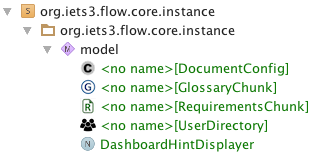
\includegraphics[width=.5\textwidth]{./figures/NewProject.png}
% \caption{A new cooling controller requirements project}
% \label{fig:newreq_proj}
% \end{figure}

After the structure of the project has been built a new hint, as shown in
figure~\ref{fig:dashboard_newreq}, proposes to
the requirements engineer defining a new requirement for the system that
includes the temperature thresholds for the functioning of the cooling system.
Note that at this point the current state of the requirements model has now
changed to ``Empty requirements model and no glossary terms defined'', as
highlighted in orange in figure~\ref{fig:dashboard_newreq} -- which now presents
a tabular view of the refinement process.
\vspace{-.6cm}
\begin{figure*}[!h]
\centering 
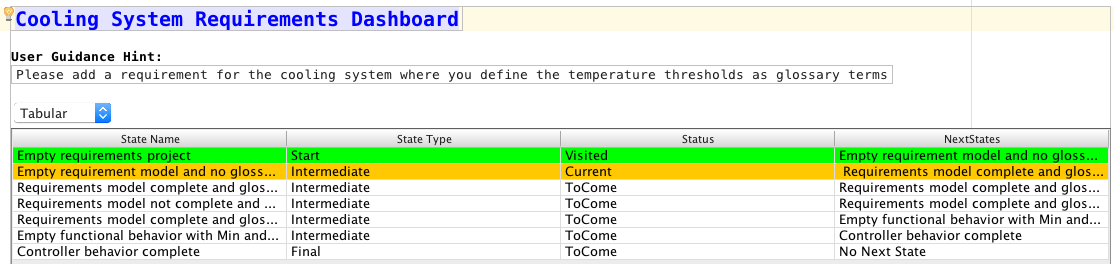
\includegraphics[width=.8\textwidth]{./figures/DefineCoolingReq.png}
\caption{The Dashboard provides a hint for adding a new requirement}
\label{fig:dashboard_newreq}
\vspace{-.6cm}
\end{figure*}

The overall desired operation of the cooling controller can be stated in the
requirement in figure~\ref{fig:new_req}, which is an instance of the
\textsf{Requirements} language.
% ``\emph{The cooling controller shall cool down the hardware board by adjusting
% the speed of the fan to an appropriate duty cycle. The duty cycle depends on the
% current temperature of the hardware and whether that temperature is increasing
% between a minimum increase value and a maximum increase value, or decreasing
% between a maximum decrease value and a minimum decrease value.}''\\
 \vspace{-0cm}
\begin{figure*}[!h]
\centering 
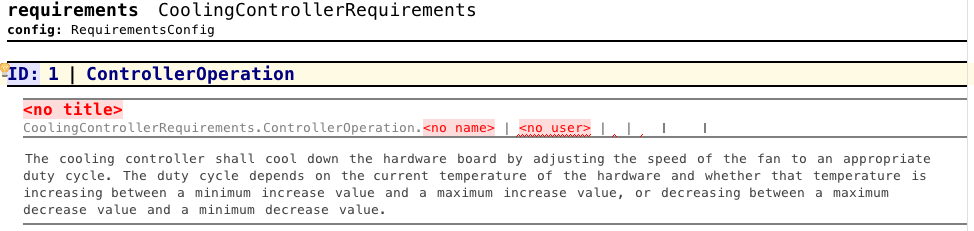
\includegraphics[width=1\textwidth]{./figures/textReqIncomplete.png}
\caption{The requirements engineer adds a new requirement}
\label{fig:new_req}
\vspace{-.6cm}
\end{figure*}

From this text the requirements engineer can then
extract minimum and maximum threshold terms using the 
MPS intention ``Extract Into Glossary'' associated to the root concepts of the
\textsf{Requirements} language. When used, this MPS intention generates in the
the project's glossary an entry with the same names as words
or sets of words selected from the text. This constitutes the first refinement
of the original abstract requirement.

% \begin{figure}[!h]
% \centering 
% 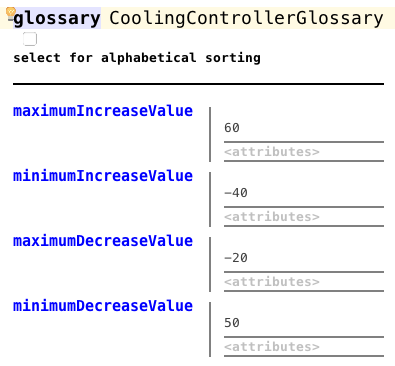
\includegraphics[width=.7\textwidth]{./figures/glossary.png}
% \caption{The glossary for the cooling controller requirements}
% \label{fig:glossary}
% \end{figure}

% Although the glossary terms for the temperature thresholds have now been
% defined, the requirement itself is still not complete, as shown by the
% dashboard's hint in figure~\ref{fig:error_dash}. This situation can be further
% investigated in detail by applying the MPS intention ``Create Error Dashboard''
% on the dashboard. In figure~\ref{fig:error_dash} a console error view
% with information about which model element currently contain which errors helps
% the user in identifying and fixing the remaining errors.
% 
% \begin{figure*}[!h]
% \centering 
% 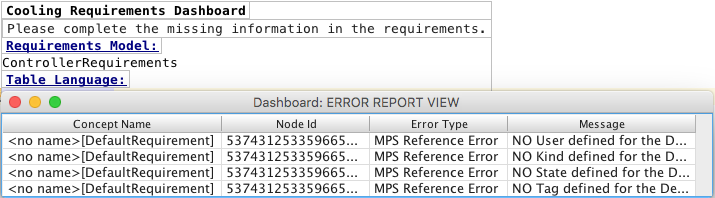
\includegraphics[width=1.7\columnwidth]{./figures/ErrorDashboard.png}
% \caption{Detailed explanation of the errors in a model}
% \label{fig:error_dash}
% \end{figure*}

The next step is to actually define the duty cycle of the fan as a function
of the current temperature of the controller board and whether the temperature
is going up or down. 
% \begin{figure*}[!h] 
% \centering 
% 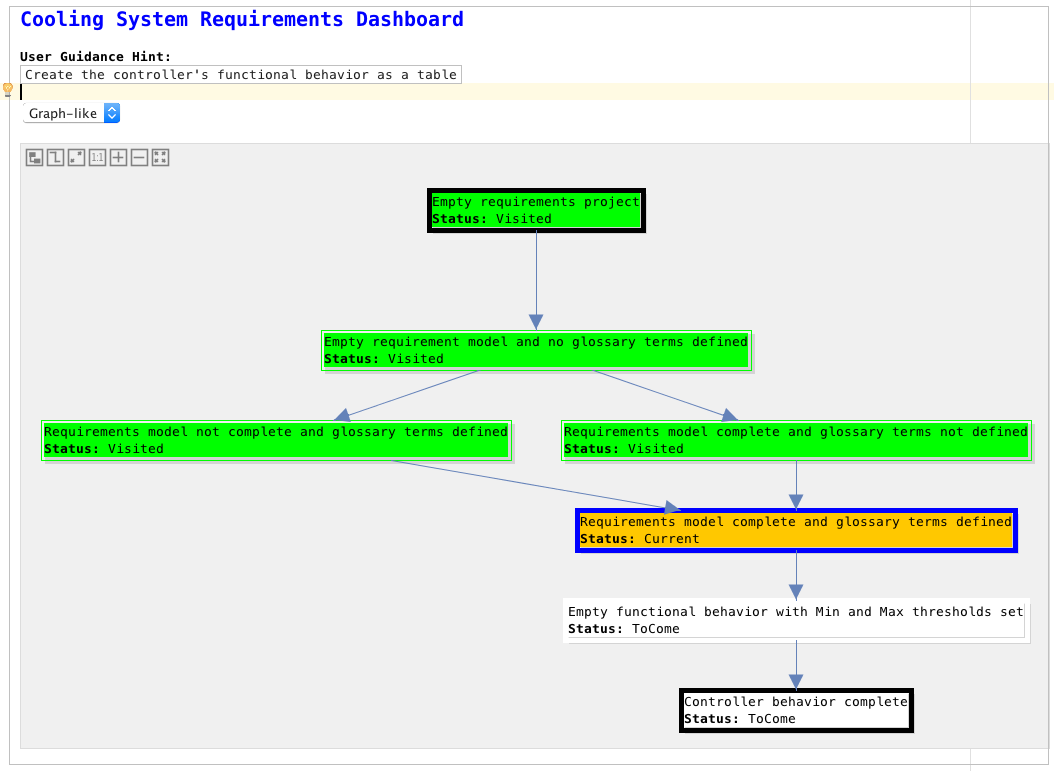
\includegraphics[width=1\textwidth]{./figures/CreateTable.png}
% \caption{The dashboard proposes creating a table to define the behavior of the
% fan controller}
% \label{fig:FAU_behavior}
% \end{figure*}
Given the hint is creational, the requirements engineer can generate an empty
table in the project model by pressing it. An example of such a table is
depicted in figure~\ref{fig:FAU_behavior_2d}.
Note that the minimum and maximum threshold values in the table are preset in
advance, as the process itself defines they should copied from the threshold values previously defined in the glossary.

The requirements engineer can now proceed to the last refinement, which is to
precisely define the behavior of the cooling fan's controller. In order to do
this it is necessary to manually insert rows in the table that define the duty cycle for
given intervals of temperature, when the temperature is going up or down. 
% \begin{figure}[!h]
% \centering 
% 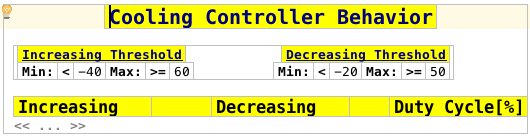
\includegraphics[width=1\textwidth]{./figures/DiehlTable.png}
% \caption{An empty table with filled in threshold values}
% \label{fig:FAU_behavior_thresh}
% \end{figure}
The \textsf{Table} language itself implements checks for completeness (all the
temperatures between the thresholds are mapped onto duty cycles) and
functionality (only one duty cycle value is given per temperature). Violations
of these properties are pointed out in the editor as red markers.
Figure~\ref{fig:FAU_behavior_2d} represents a filled in table holding, for
non-disclosure reasons, a fictitious complete behavior of the fan's controller.
In the figure the 2D-graph representation of the table is also shown, and it can
be produced by applying the “Visualize Graph” MPS intention to the table.
\begin{figure*}[!h]
\centering
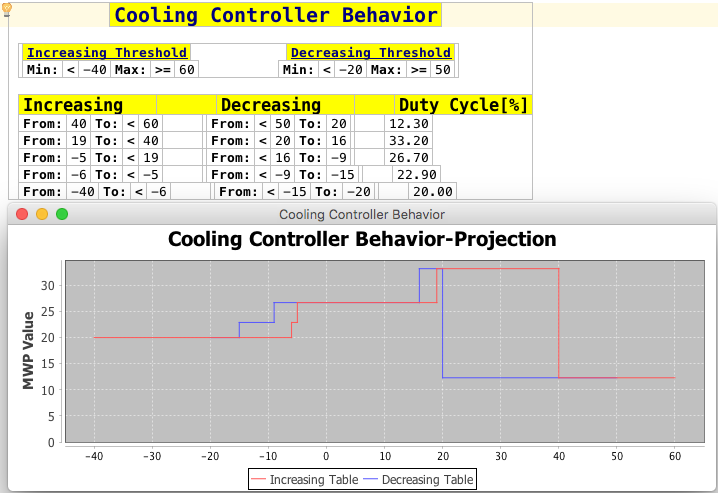
\includegraphics[width=.7\textwidth]{./figures/DiehlTableAnd2DGraph.png}
\caption{An filled in table and associated 2D visualization of the defined
function}
\label{fig:FAU_behavior_2d}
 \vspace{-1cm}
\end{figure*}

% \saad{Text moved from model level to instance level} Our example case study
%  is inspired by one of our industrial partners (i.e., Diehl aerospace) that builds cooling systems for airplane hardware. We have abstracted an example requirement, where the user is required to correctly build requirements leading to a description of the expected behavior of a cooling system. The abstract requirement that requires to be built and refined by the user contains the following,
% \begin{itemize}
%   \item the minimum and the maximum temperature thresholds of the controller
%   boards,
%   \item the behavior of the cooling system that it increases or decreases the
%   duty cycle of the cooling unit based on the current temperature of the
%   controller board and
%  \item whether the temperature is increasing or decreasing. 
% \end{itemize}

The running example we have described in this paper can be downloaded
at~\cite{coolingControllerProcess} as an MPS project. Another case study of
using our framework is available at~\cite{earsctrlProcess}, where we have
designed a process to assist the user in building natural langage-like
requirements for embedded controllers. Note that
both~\cite{coolingControllerProcess,earsctrlProcess} are GitHub repositories
that contain not only MPS projects, but also additional information about how to
install those projects as well and pointers to videos demonstrating all the
steps and artefacts we explicitely or implicitely describe in this paper.
 \vspace{-.6cm}
  



